\documentclass[11pt, a4paper, oneside]{article}
\usepackage[ngerman]{babel}
\usepackage{worksheet}

\begin{document}
	\author{L. Bung}
	\title{Martin-Notation}
	\subject{SAE}
	\class{E2FI}
	\maketitle
	
	Neben der üblichen Notation von Entity-Relationship-Modellen (die nach dem Entwickler der ER-Diagramme als Chen-Notation benannt ist), ist auch die \textbf{Martin-Notation} (oder auch Krähenfuß-Notation) eine weit verbreitete Darstellungsmöglichkeit von ER-Modellen.
	
	Hierbei wird statt der Bezeichnung $1$ bzw. $n$ die Kardinalitäten $0$ (Null), $|$ (Eins) und $<\!\!\!\!\!\!-$ (beliebig viele) verwendet.
	
	\begin{figure}[H]
		\centering
		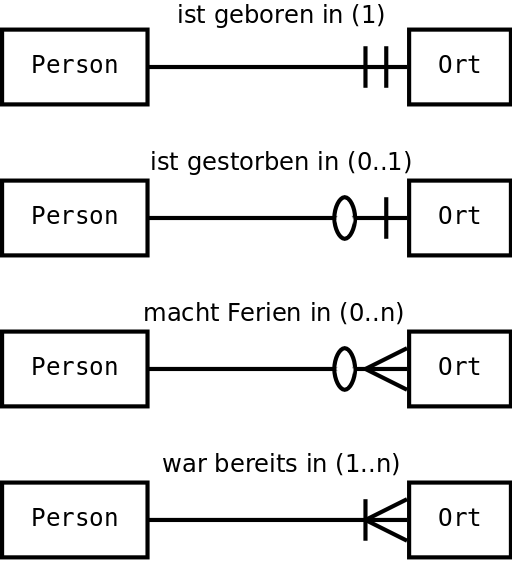
\includegraphics[width=.5\textwidth]{Martinnotation.png}
		\caption{Beispiele für Verwendung der Martin-Notation\protect\footnotemark}
	\end{figure}
	\footnotetext{\url{https://de.wikipedia.org/wiki/Datei:MartinOdell.png}}
	
	Hierbei hat jede Seite der Relation zwei Kardinalitätsangaben:
	Eine Obergrenze und eine Untergrenze.
	Das Resultat ist ein deutlich genaueres Modell, was jedoch aufgrund der einfachen Notation immer noch gut lesbar ist.
\end{document}